\chapter{Apendice B}

\section{ODROID}
El modelo XU-4 cuenta con las siguientes especificaciones:~\cite{hardkernel2017}
\begin{itemize}
    \item \textbf{Procesador}\\
    Samsung Exynos5422 Cortex™-A15 2Ghz and Cortex™-A7 Octa
    core CPUs con Mali Mali-T628 MP6 GPU.\\
    Es un procesador mobil que fue lanzado en 2014 por Samsung para su celular S5.
    \item \textbf{Almacenamiento}\\
    Hay dos tipos de almacenamiento de el sistema operativo. El primero es usando
    una microSD y el segundo es utilizando un modulo eMMC.
    \item \textbf{Alimentación}\\
    Es necesario alimentar con 5V y con un minimo de 4A para su optimo funcionamiento.
    \item \textbf{Perifericos}
    \begin{itemize}
        \item USB hosts
        \item HDMI
        \item Ethernet RJ-45
        \item GPIO (Entradas y salidas de SPI,ADC e IRQ)
        \item Comunicación serial
        \item USB 3.0
    \end{itemize}
    
\end{itemize}
\begin{center}
    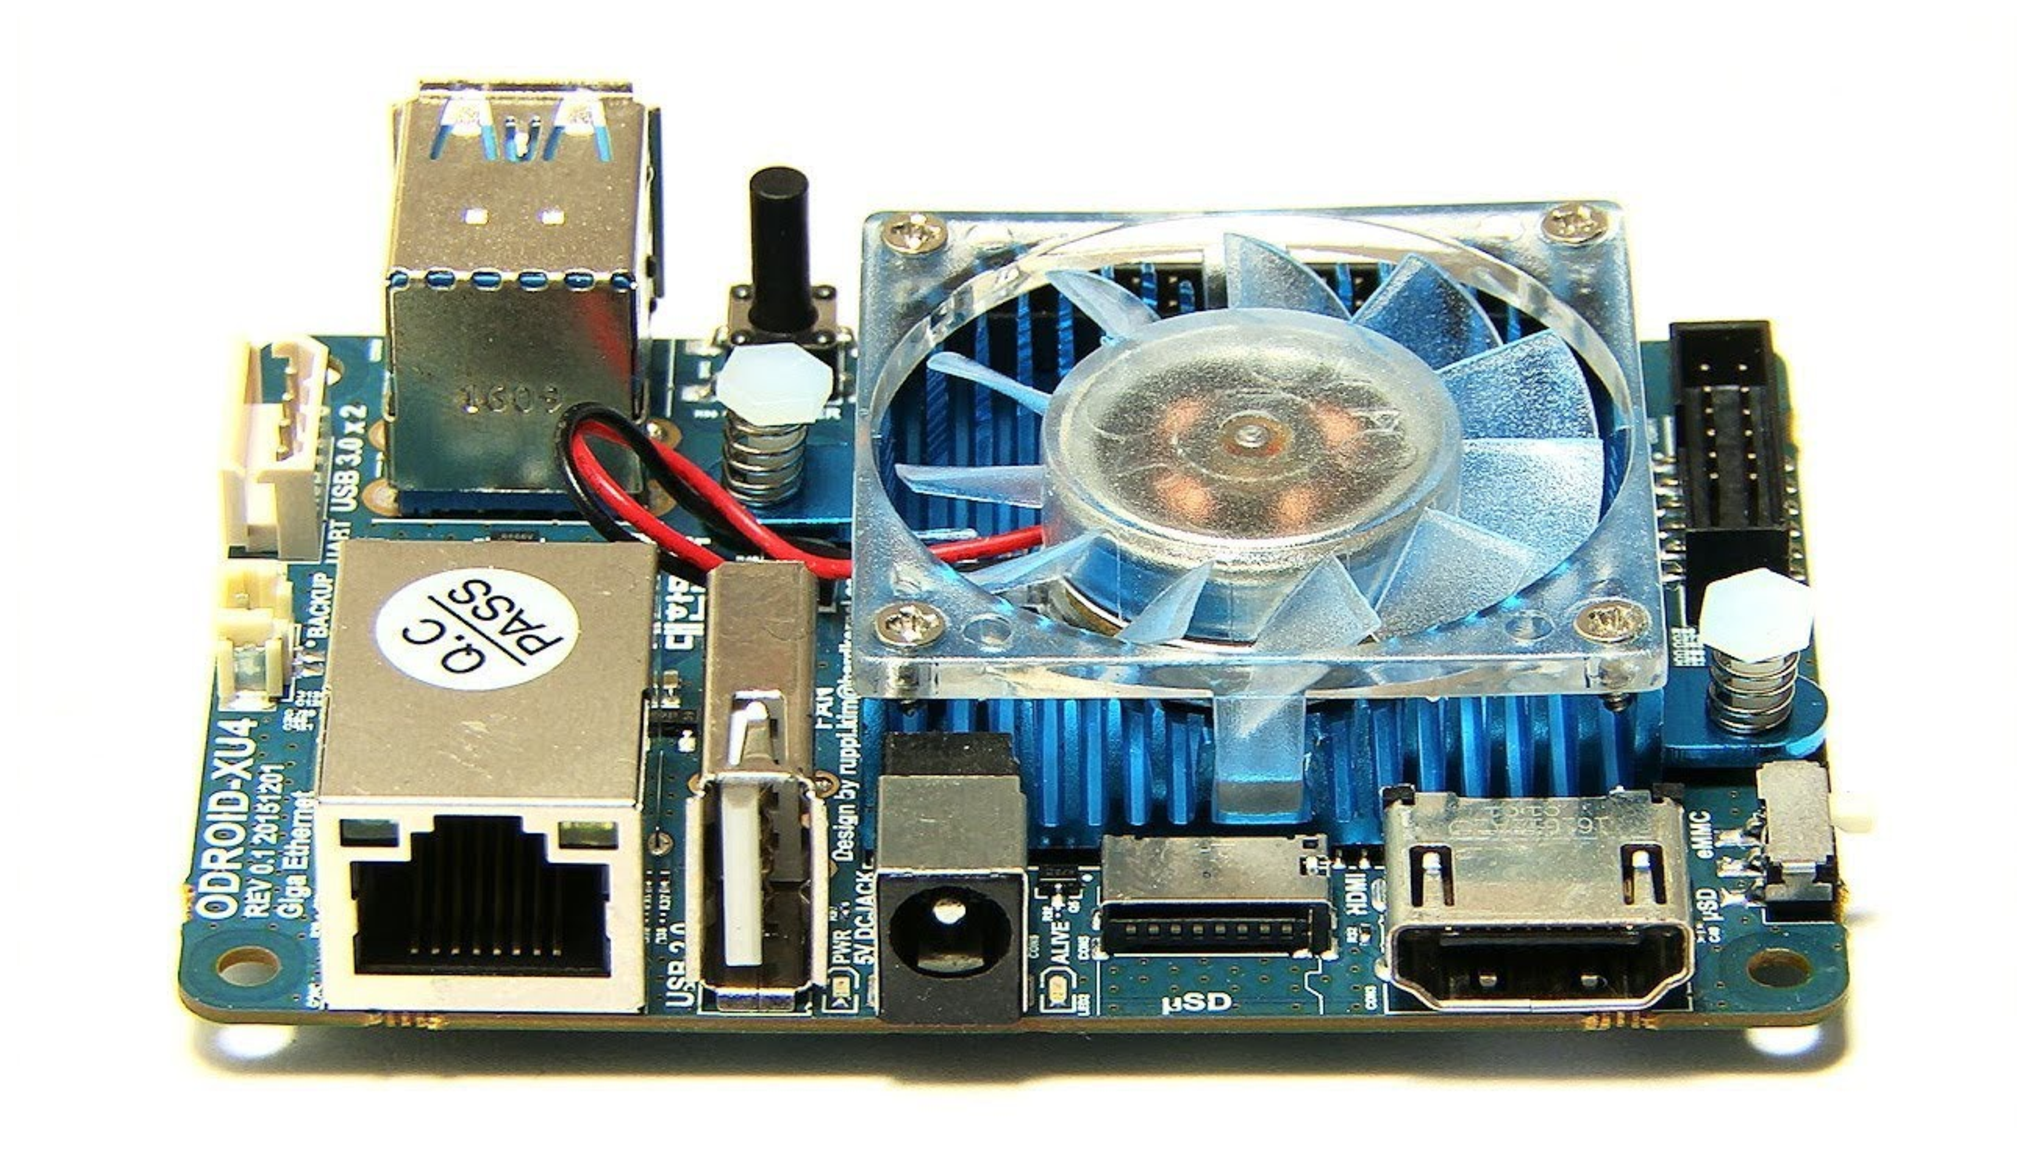
\includegraphics[width=0.55\textwidth]{Contenido/Back/Apendices/ApendiceB/Fig0.eps}
    \captionof{figure}{Odroid XU-4}\label{Fig5}
\end{center}

\section{Atmega328P}
Es el microchip que esta embebido en el microcontrolador Arduino UNO. Cuenta con las siguientes características:
\begin{itemize}
    \item Program memory size: 32KB
    \item SRAAM: 2,048 B
    \item serial communication, I2C y SPI
\end{itemize}

La elección de este microchip es por su compatibilidad con ROS-Serial, y además por su amplia documentación.